\documentclass[../main.tex]{subfiles}
\graphicspath{{\subfix{../images/}}}

\begin{document}
	
\chapter{Literature Review}

What I need to do in the literature review is an introduction, body and conclusion. The introduction should be an overview of the topics that I am going to talk about, and probably introduce the research motivation.

\section{Introduction}

Additive manufacturing, also known as 3D printing, is a manufacturing process in which parts are built by stacking layers of material on top of each other until the desired geometry is created. In particular, powdered-bed fusion is a type of additive manufacturing in which the base material is composed of a metallic powdered. A bed is then filled with this powder, and a high-powered laser or electron beam is utilized to selectively add heat to locations of this powdered metal, thus melting it. As the melted portions cool, it leaves a layer of solid material, and the whole component is then built layer by layer in this manner. If a laser is used for manufacturing, the process is then known as laser powder bed fusion (LPBF).

PBF involves the layer-by-layer addition of material in which a heat source selectively melts and fuses regions of a powder bed to form a solid structure. When the material is melted and fused by using a laser, the process is called selective laser melting (SLM). The starting point of selective laser melting is a 2D computer-assisted design (CAD) model, which is sliced into 2-dimensional pieces, and later uploaded to an SLM machine. The machine then uses the laser to melt layers of powder following the information of the sliced model. At the end of each slice, the layer is left to cool down and solidify, and a new layer of powder is evenly distributed using a coater, and the melting process begins anew, until the final geometry has been reached \cite{valinoAdvances3DPrinting2019}. The part is then removed from the powder bed where it might then undergo different post-processes, such as removal of supporting structures, heat treatment, or any other additional or removal of material to achieve the required dimensions and tolerances. 

Additive manufacturing in general allows for the creation of parts with complex geometries that would otherwise be difficult, time-consuming or too costly to manufacture with other more traditional means of manufacturing such as machining or casting. This can be compared with the manufacture of prosthesis using traditional manufacturing, which relies on the high-volume production of standardized parts and shapes. Due to the ease of creating parts with complex geometries and with shorter lead times, additive manufacturing has had a growing interest from the medical industry for the creation of custom-made implants tailored to an individual patient's anatomy \cite{marshTrendsDevelopmentsHip2021} \cite{narraAdditiveManufacturingTotal2019}. Additionally, this benefit of creating customized parts also leads to an improvement of patient comfort and better outcomes in orthopedic and surgical applications, as well as enhancing surgical precision and reducing complications of post-operative care \cite{mobarakRecentAdvancesAdditive2023} \cite{pathak3DPrintingBiomedicine2023}.

Despite its advantages in creating components with complex free-form 3D geometry, SLM still faces many challenges that limit its application and development. Some of these challenges are related to the development of excessive deformation, thermal stresses, and other mechanical defects such as delamination, distortion and microcracks that result from the great thermal gradients that occur within the component as it is being built, caused by the high heating and cooling rates inherent in the process \cite{jonaetPredictionResidualStress2021}.

Additionally, even though additive manufacturing is a viable alternative for the production of complex-shaped components, its cost can still remain high due to machine, material and process-level expenses. In particular, as a means of creating medical implants for knee-replacement therapy, the high cost of AM limits its usage for revision procedures, i.e. second or third procedures in which the objective is to replace a failed or uncomfortable component \cite{narraAdditiveManufacturingTotal2019}. To solve the problem of high material costs, Laureijs et al. \cite{laureijsMetalAdditiveManufacturing} have identified that one of the main driving costs is the price of the powder price. One of the viable options to drive down the price of prosthesis created using additive manufacturing would be to reduce the amount of scrap material involved in the process. Scrap material in additive manufacturing results from discarding the support structures that the part requires as well as any addition or removal of material to the part in post-processing steps to ensure that the part is maintained within tolerances \cite{laureijsMetalAdditiveManufacturing}.

The support structures alluded to in the previous paragraph refer to the structures that are built alongside the manufactured component that serve to stabilize it during the printing process. These structures are used to aid with supporting overhang areas, which are defined as areas in the structure that are almost horizontal. Support structures can also facilitate the remove of the part from the base plate and other workpieces, and can also aid with thermal diffusion or prevent residual stresses caused by thermal gradients \cite{chungpei-hsuStudyLatticeSupport2024}. 

The design of support structures in additive manufacturing is thus an important consideration, with many factors affecting how the support structure will be built. A well optimized and design support structure will enable the part to be realized, while at the same time using the least amount of material possible to obtain a specified objective. Thermal and mechanical requirements are usually at the forefront of support structure design as they have a direct effect on the quality of the component, although there might be other considerations for the design, such as ease of removability, build time, and material efficiency. Additionally, large portions of surfaces that are almost horizontal and that are unsupported during manufacturing tend to be heavily distorted after manufacturing \cite{allaireOptimizingSupportsAdditive2018}. At overhang regions, support structures are also required to be as stiff as possible to withstand the weight of the part itself and prevent it from distorting during the building process \cite{kuoSupportStructureDesign2018} \cite{kumarTailoredSupportStructures2020}.Another important factor that impacts the design of support structure is the structure's performance to transfer heat away from the build component, since high thermal conduction can improve the cooling process during fabrication, which helps prevent issues caused by excessive thermal deformation such as thermal residual stresses, thermal dilation, cracks or warping \cite{allaireOptimizingSupportsAdditive2018} \cite{zhouTopologyOptimizationThermal2019}.

Topology optimization is a method that is well-suited for the creation and optimization of shapes that satisfy specific constraints while realizing certain objectives \cite{bendsoeTopologyOptimization2002}, and is a well-known technique that has been obtaining more interest from the additive manufacturing community for both the design of the components themselves and for their support structures in additive manufacturing. Topology optimization has been studied for designing parts that either have as little overhang surfaces as possible, thus requiring less supporting structures, or for designing parts that are self-supporting, thus requiring no supporting structures at all. Although this aid considerably in reducing the amount of material used, these approaches do not take into consideration other effects such as the thermal dissipation of the component, or require changing the geometry of the component, thus impacting its functionality \cite{yeTopologyOptimisationSelfsupporting2023}. Changes in the geometry of the component might also impose geometrical constraints that can restrict the part's performance \cite{langelaarTOPOLOGYOPTIMIZATIONADDITIVE2016}. Therefore, instead of using topology optimization to change the shape of the part, much research has been made to apply topology optimization to the design of the support structure itself.

Since topology optimization is one of most popular methods for the design of support structures and the central idea used for this thesis, the following section will consist of an overview of the main ideas and implementation of topology optimization.

\section{Topology optimization}

\subsection{Formulation}
Topology optimization is an optimization technique that seeks to find the optimal shape within a volume that satisfies certain governing equations while at the same time satisfying specific constraints. This technique is usually utilized for the design of structures with no preconceived shape. Mathematically speaking, topology optimization seeks to find the optimal distribution of a design variable $\rho$ within a design domain. The placement of $\rho$ will also obey certain governing equations that are valid within the domain, and the existence of this distribution of $\rho$ will also depend on a certain objective that is wished to be minimized, alongside other constraints that might be imposed in the system. A classical example of topology optimization is the so called binary compliance problem, in which regions of solid and void material are distributed inside a volume to design a structural component that will be able to withstand certain loads applied to its boundaries, but that will have the least amount of deformation possible, while only using a certain fraction of the design volume, or keeping the total weight of the structure withing a certain limit. We can express this specific problem mathematically as:

\begin{align} 
  min: & \hspace{0.5cm} c(\bm{\rho}) = \bm{F}^T \bm{U}  \label{eq:to1} \\
  s.t.: & \hspace{0.5cm} \bm{K}(\bm{\rho})\bm{U} = \bm{F}  \label{eq:hooks}\\
        & \hspace{0.5cm} V = \sum _{i \in \Omega} \rho_i v_i \leq V_c \label{eq:volfrac} \\ 
        & \hspace{0.5cm} 0 \leq \rho_{min} \leq \rho_i \leq 1 \label{eq:to4}
\end{align}

where in equation \ref{eq:to1} the objective function that is to be minimized is given by $c(\bm{\rho}) = \bm{F}^T \bm{U}$, where $\rho$ takes the value 0 or 1 depending on whether our small region in space is empty or contains material, $\bm{U}$ is the displacement of piece of material and $\bm{F}$ is the force applied to it. This quantity is referred to as compliance, and physically it is the inverse of the stiffness of the structure. The deformation of this material in the design domain is controlled by Hooke's Law, which is shown in equation \ref{eq:hooks}. $\bm{K}(\bm{\rho})$ is defined as a global stiffness matrix \cite{hornbergerFiniteElementMethod2005}
\begin{equation}
  \bm{K}(\bm{\rho}) = \sum_{i \in \Omega} \bm{K}_i(\rho_i)
\end{equation}

where the design domain $\Omega$ is split into $i$ regions, and $\rho_i$ is the density at each region $i$, and we assemble all those densities into the vector $\bm{\rho}$. 

More generally, the formulation of topology optimization can be written as a minimization problem over a domain subject to one or more constraints, where the quantity that is being minimized is called the objective function. The quantity that is being minimized could in turn be composed of several smaller objectives, each with its own relative weight or importance with respect to the final solution. The minimized quantity is also written as a function of the design variables, which in most topology optimization problems refer to the amount of material that is present in a specific region of the design domain. Additionally, we might impose an upper limit of the total amount of volume used. This was shown in equation \ref{eq:volfrac}, where the maximum allowed volume fraction of the design domain $\Omega$ is denoted as $V_c$. Mathematically, the generalized problem of topology optimization can be formulated as follows:

\begin{align}
  find: & \hspace{0.5cm} \rho_i, \hspace{0.5cm} (i = 1, 2, ..., n)  \nonumber \\ 
  min:  & \hspace{0.5cm} X_{obj} = w_1 O_1 + w_2 O_2 + ... + w_m O_m  \nonumber \\ 
  s.t.: & \hspace{0.5cm} \text{governing equations}  \\ 
        & \hspace{0.5cm} V = \sum _{i \in \Omega} \rho_i v_i \leq V_c \nonumber \\ 
        & \hspace{0.5cm} 0 \leq \rho_{min} \leq \rho_i \leq 1, \hspace{0.5cm} (\rho_1, \rho_2, ... \rho_n \in \Omega) \nonumber \\
        & \hspace{0.5cm} w_1 + w_2 + ... + w_m = 1 \nonumber 
 \end{align}

\subsection{Homogenization and SIMP}
Unfortunately, the formulation above suffers from a major problem. Stated as is, the problem above is well-known to be ill-posed \cite{kohnOptimalDesignRelaxation1986}, as it is possible to obtain a chattering design with an infinite number of holes of infinitesimal size, thus rendering this compliance problem to be unbounded \cite{liuEfficient3DTopology2014}. To remedy this situation, several approaches have been proposed in the literature. One approach to control the chattering design is ensure that the total perimeter of the resulting structure has an upper bound \cite{haberNewApproachVariabletopology1996} \cite{jogTopologyDesignStructures2002}, but this e method suffers from several complications in implementation, and small variations in the parameters of the algorithm can lead to wildly different designs of the final structure \cite{jogTopologyDesignStructures2002}.

A different alternative would be the utilization of a homogenization method \cite{bendsoeOptimizationStructuralTopology1995}, \cite{allaireShapeOptimizationHomogenization2002} \cite{suzukiHomogenizationMethodShape1991} in which the binary representation of the material within the design domain is relaxed and intermediate values of densities are allowed, instead of just allowing empty and filled-values. One of the difficulties with using the homogenization method is how to interpret the intermediate densities of the material. In topology optimization problem involving the design of fluid flow media, the minimum value of the density could be interpreted as a fluid, the maximum value could be interpreted as a solid, while intermediate values could be interpreted as porous media \cite{pietropaoliThreedimensionalFluidTopology2019}. In structural problems, intermediate values could be interpreted as periodic composite materials with high-resolution microscopic features \cite{groenHomogenizationbasedTopologyOptimization2018} \cite{alexandersenTopologyOptimisationManufacturable2015}, materials that are composed of lattice structures \cite{allaireTopologyOptimizationModulated2019}, or even complex structures consisting of anisotropic fiber-reinforced composite materials \cite{kimTopologyOptimizationFunctionally2020}. Although the homogenization method is successful in solving the chattering design problem, validation of the resulting topologies using most Finite Element Method (FEM) software is very computationally expensive, since the resulting microstructures requires very fine meshes with high number of elements and nodes \cite{kimComputationalHomogenizationAdditively2022}. Additionally, the use of microstructures can also lead to stress amplifications which need to be managed appropriately to avoid regions of high stress concentration that might compromise the stability or functionality of the manufactured part \cite{allaireTopologyOptimizationMinimum2004}. It is also worthy of note that when this method was introduced back in the 1980's, manufacturability of components designed with the homogenization method was not feasible, as it was very difficult to manufacture components with microstructures or lattices. Nevertheless, the recent progress of additive manufacturing has revived the interest for structures with microstructures due to their newfound manufacturability \cite{allaireHomogenizationMethodTopology2019}.

A simpler method that tries to avoid the complications of homogenization theory is the Solid Isotropic Material Penalization method (SIMP), which utilizes yet another continuous density function. The main point of SIMP is to apply a power-law interpolation function to the material density, with the objective to penalize intermediate densities and drive them to their extreme values of void and full material. \cite{bendsoeOptimalShapeDesign1989} \cite{rozvanyGeneralizedShapeOptimization1992}. This method was beneficial at the time this method was being developed in the late 80's and 90's, since as previously mentioned, it was yet fairly difficult to manufacture parts with complicated microstructures, and thus methods that drove densities to a binary result of void and material were preferred. Additionally, since the implementation of this method is simpler and less computationally intensive than homogenization, many modern FEM software use SIMP for topology optimization \cite{SIMPMethodTopologyb}.

To understand its implementation, let us return to the problem of the design of a support structure by minimizing its compliance (equations \ref{eq:to1} - \ref{eq:to4}). Since the material density is allowed to take intermediate values, the same applies for the structure's mechanical properties, and therefore Young's modules could be computed using the following power law:

\begin{equation}
  E_i = E_i(\rho_i) = \rho^p_i E_i,
  \label{eq:young_simp}
\end{equation}

where $E_i$ is the modulus of elasticity at a region i of the design domain $\Omega$, $\rho_i$ is the density field at that region $i$, $E_0$ is the modulus of elasticity of the solid material and $p$ is the penalization factor that tries to drive the density towards its binary void and solid values. However, since the SIMP method is usually used in conjunction with FEM to solve for the density distribution, it is required to avoid void material configurations that would result in singularities during the numerical computation steps. Instead, we can rewrite equation \ref{eq:young_simp} as:

\begin{equation}
  E_i = E_i(\rho_i) = E_{min} + \rho_i^p (E_0 - E_{min}),
  \label{eq:simp_modified}
\end{equation}

in which the addition of the $E_min$ avoids singularities, and $E_0$ can be chosen to be small to represent regions of void material.

\subsection{Filtering techniques}

Unfortunately, usage of the SIMP method as stated in \ref{eq:simp_modified} can also result in checkerboard patterns or might add very thin details that are comparable in size to the mesh size, causing the final result to converge to a very different topology depending on the of the length scale of the mesh \cite{wangProjectionMethodsConvergence2011a}. One of the possible techniques in the literature used to solve this problem is the use of filtering techniques on the density field. The main idea of these filtering techniques is to modify the density field at a point so that it becomes a weighted average of the densities of its neighboring points. Using this idea, a new filtered density field can be mathematically defined using the following equation \cite{liuEfficient3DTopology2014}:

\begin{equation}
  \tilde{\rho_i} = \frac{\sum_{j \in N_i} H_{ij} v_j \rho_j} {\sum_{j \in N_i} H_{ij} v_j},
\end{equation}

where $\rho_j$ is the density field at a small region $j$ of the design domain $\Omega$,$v_j$ is the total volume of the region in consideration, and $N_i$ is a neighboring region around $v_j$. The term $H_ij$ is the weighing function, and it is analogous to a kernel, or convolution matrix, that is used in image processing applications to modify the properties of a pixel based on its surroundings, and that is typically used to blur, sharpen, emboss or perform other transformations to the image used (i.e. an image filtering function). $H_{ij}$ could be defined as a function of the distance between the element and neighboring elements, and should be chosen so that it is linearly or exponentially decaying away from the element. A possible weighting function could be calculated as 

\begin{equation}
  H_{ij} = \max(1 - \frac{(x_j - x_i)^2 + (y_j - y_i)^2)}{r}, 0),
  \label{eq:weighfunction}
\end{equation}

where in this example, the design domain is two-dimensional, and $x_i$ and $y_i$ is the point in consideration, and $r$ is the radius of filtration. In other literature, equation \ref{eq:weighfunction} is also expressed as \cite{liuEfficient3DTopology2014} 

\begin{equation}
  H_{ij} = r -  dist(i, j),
\end{equation}

Where $dist(i,j)$ contains all the neighboring points $j$ within a distance r of point $i$.

Another alternative to using equation \ref{eq:young_filtered} is to instead define the filter implicitly using a solution to the Helmholtz partial differential equation (PDE) using homogeneous Neumann boundary conditions that are imposed on the boundary of the design domain \cite{lazarovFiltersTopologyOptimization2011}

\begin{align}
  -r^2 \nabla ^2 \tilde{\rho} &+ \tilde{\rho} = \rho \label{eq:Helmholtz}\\ 
 \frac{\partial{\tilde{\rho}}}{\partial {\bm{n}}} &= 0 \nonumber,
\end{align}

where $r$ is the filter radius. The solution of this equation is a function that decays monotonically as is desired, and also preserves the volume of the design domain after the filtering process is completed. Additionally, equation \ref{eq:Helmholtz} can be solved within the same finite element solver that is utilized for the solution of the whole topological optimization problem, and it requires no extra information beyond the mesh connectivity around each volume or mesh element \cite{lambeTopologyOptimizationUsing2018}. It is also important to note that when the Helmholtz filter or any other filtering function is implemented into a finite element solver, the filter radius $r$ must be bigger than the mesh edge size in order to obtain mesh independent results \cite{PerformingTopologyOptimization}.

\subsection{Threshold projection}

Even though filtering is effective at solving the checkerboard design pathology, the structure that is designed can also suffer from intermediate density values. To try and converge these intermediate values into a void/solid configuration, projection functions can be used to project the results of the filtered density field into 0/1. One method proposed by Xu et al. \cite{xuVolumePreservingNonlinear2010} is a volume-preserving, modified continuous Heaviside function which takes the following form

\begin{equation}
  \bar{\tilde{\rho}} = \begin{cases}
    \eta [e^{-\beta (1 - \tilde{\rho} / \eta)} - (1 - \tilde{\rho} / \eta) e^{- \beta}] & 0 \leq \tilde{\rho} \leq \eta\\ 
  \begin{split}
    (1-\eta)[& 1 - e^{-\beta (\tilde{\rho} - \eta) / (1 - \eta)} \\ 
             & + (\tilde{\rho} - \eta) e^{- \beta} / (1 - \eta )] + \eta
  \end{split} & \eta \le \tilde{\rho} \leq 1.
\end{cases} 
  \label{eq:heaviside_filter}
\end{equation}

In equation \ref{eq:heaviside_filter} $\bar{\tilde{\rho}}$ is the new projected density value, $\tilde{\rho}$ is the filtered density value obtained from the filter function explained in the previous section, $\eta$ is a parameter that will determine where the cutoff point between the 0/1 values will be made in the x-axis, and $\beta$ will determine how fast the transition from 0/1 will be. Figure \ref{fig:heaviside_filter} has been included to aid the reader in understanding how the parameters affect the shape of the function.

\begin{figure}
  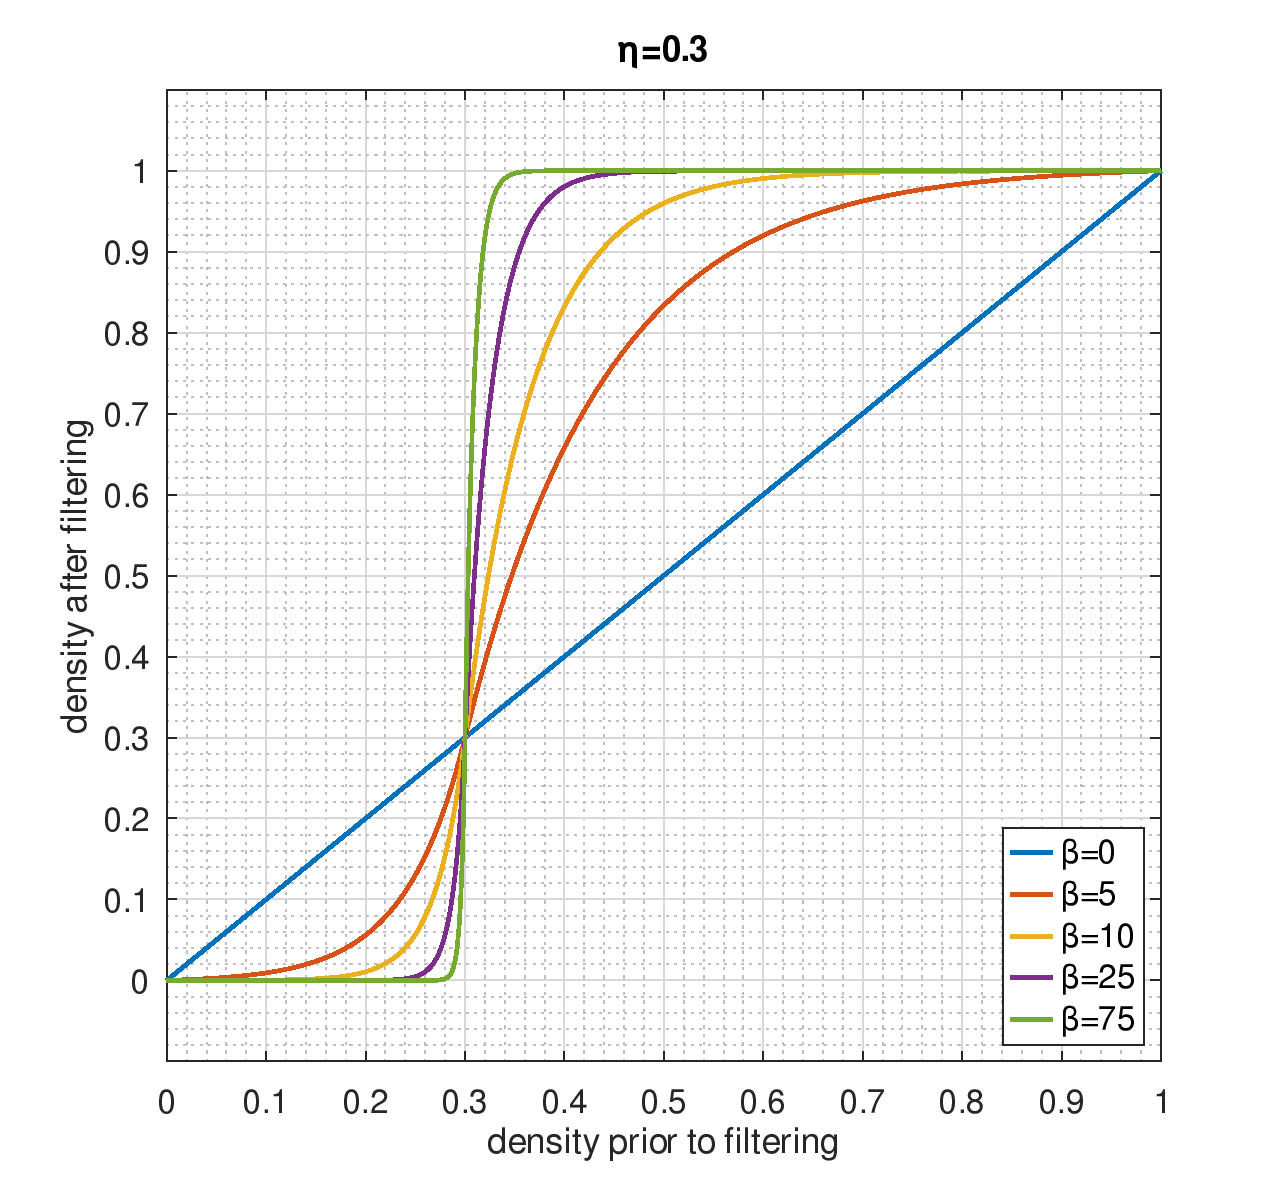
\includegraphics[width=.46\textwidth]{eta03.png} \hfill
  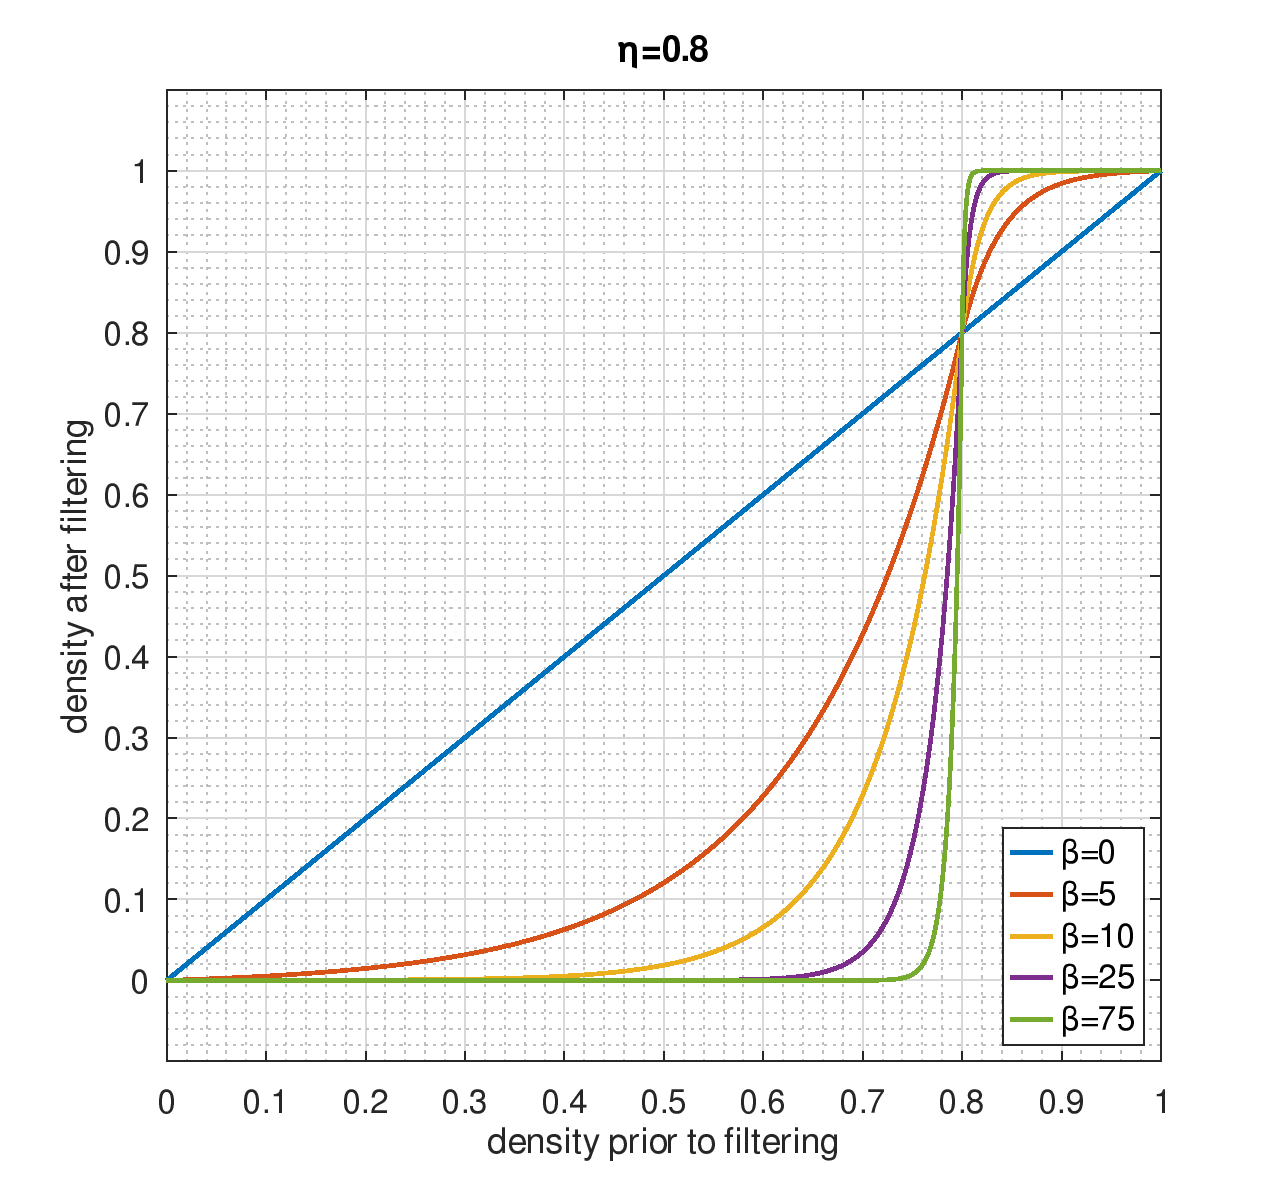
\includegraphics[width=.46\textwidth]{eta08.png} \hfill
  \caption{Smoothed modified Heaviside filters with $\eta$ = 0.3, $\eta$ = 0.8, and different values of $\beta$.}\label{fig:heaviside_filter}
\end{figure}

Although the expression in equation \ref{eq:heaviside_filter} is successful in project the filtered density values, it can be replaced by a simpler and shorter expression utilizing the hyperbolic tangent function \cite{wangProjectionMethodsConvergence2011a}

\begin{equation}
  \bar{\tilde{\rho_i}} = \frac{tanh(\beta \eta) + tanh(\beta(\tilde{\rho}_i - \eta))}{tanh(\beta \eta) + tanh(\beta (1 - \eta))} 
  \label{eq:tanh_filter}
\end{equation}

Equation \ref{eq:tanh_filter} has the added benefit of computing the 0/1 projection faster, and in the limit as $\beta \xrightarrow {} \infty$ it yields the same result as equation \ref{eq:heaviside_filter}. Plots of this equation are shown in figure \ref{fig:tanh_filter}.

\begin{figure}
  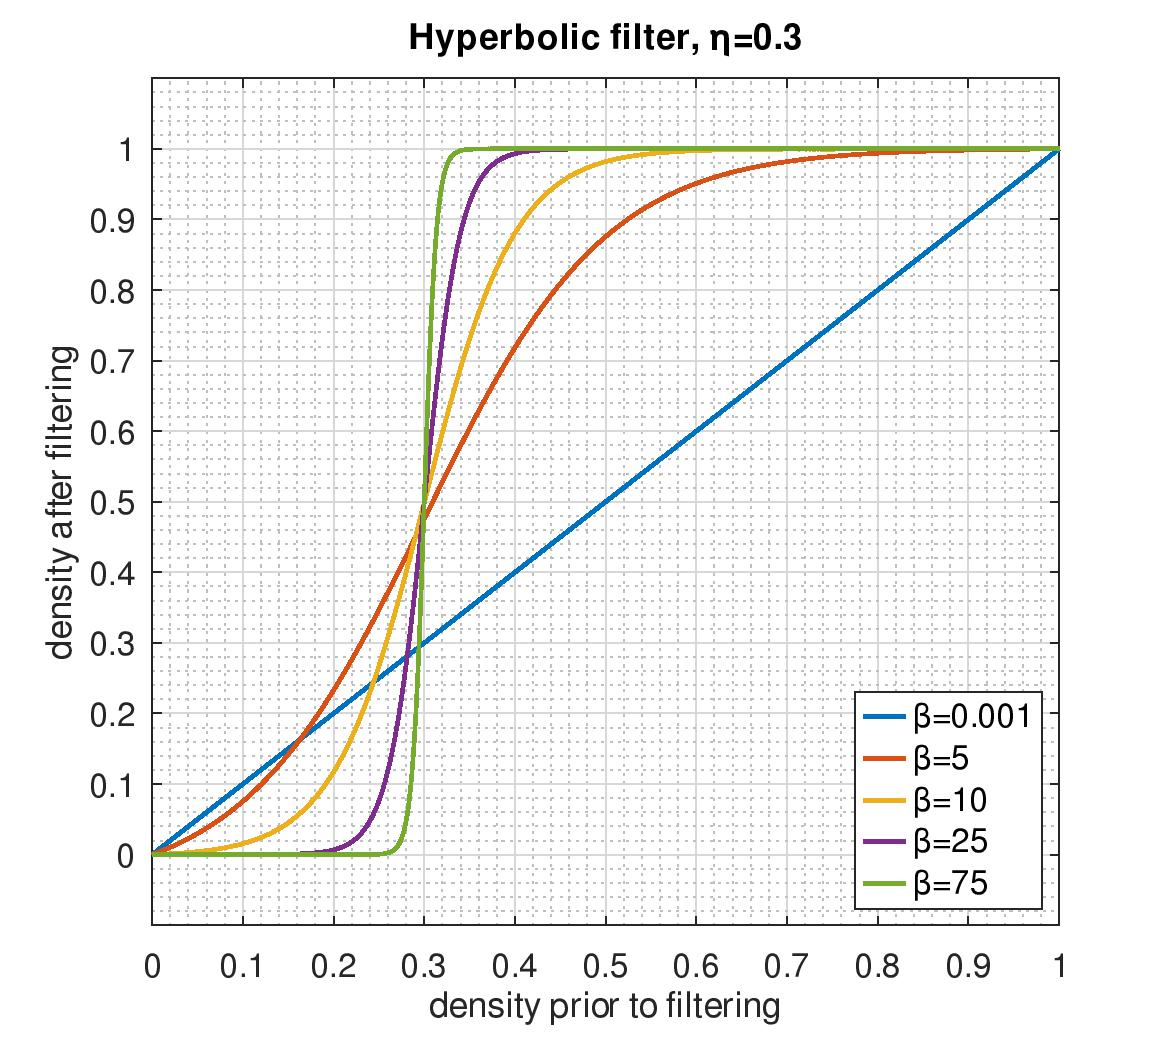
\includegraphics[width=.46\textwidth]{hyp3.jpg} \hfill
  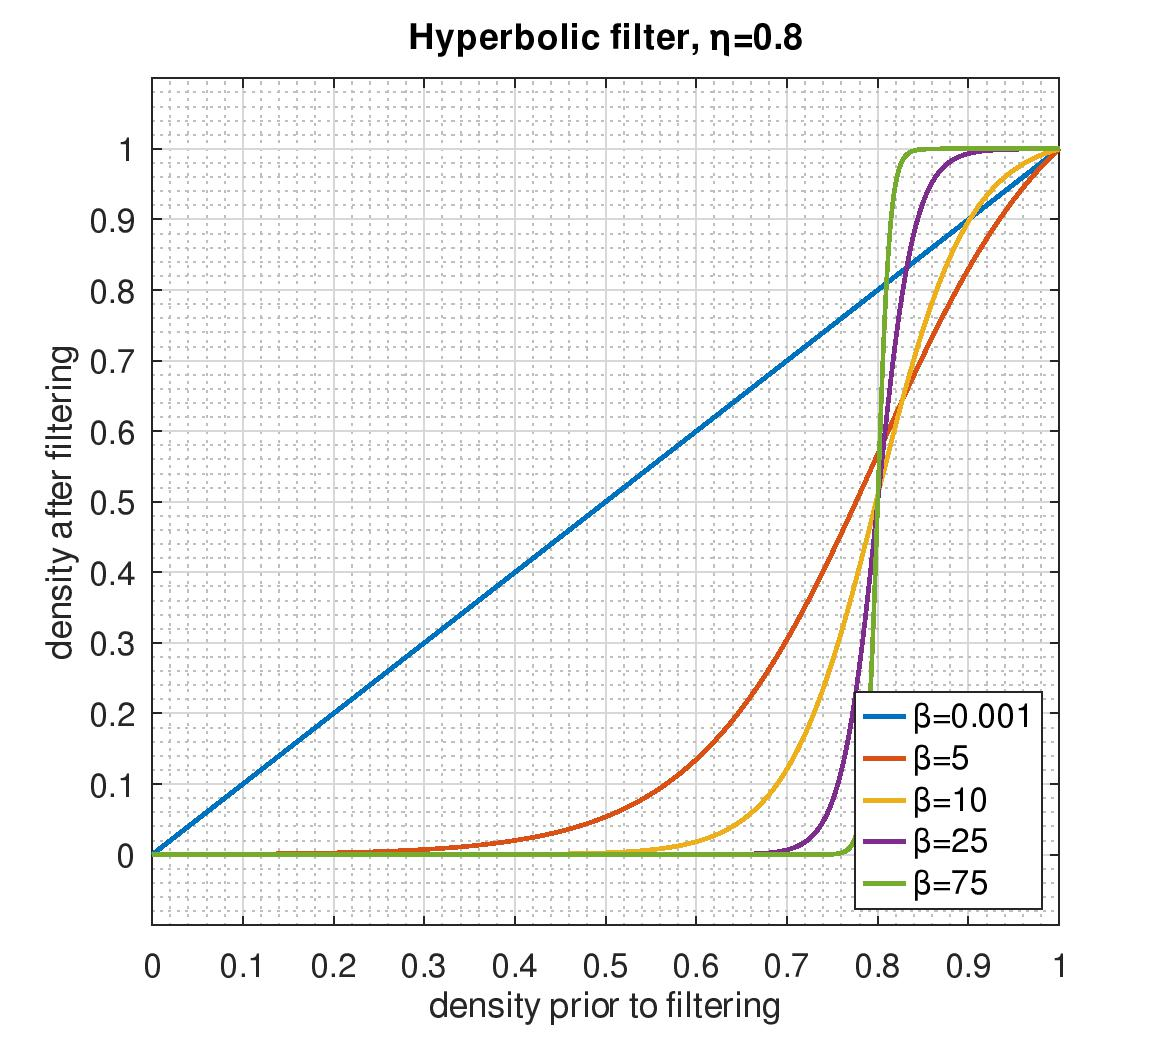
\includegraphics[width=.46\textwidth]{hyp8.jpg} \hfill
  \caption{Hyberbolic tangent filter function with $\eta$ = 0.3, $\eta$ = 0.8, and different values of $\beta$.}
  \label{fig:tanh_filter}
\end{figure}

\todo{the part below should be the last part, since the density function that is used to calculate physical properties has to be the final density function after filtering and projecting}

\subsection{Final formulation of the topology optimization problem}
When a density filter is applied, the mechanical properties of the structure, such as Young's modulus or thermal conductivity, also become a function of the filtered function. For example, in the context of the structural problem described by equations \ref{eq:to1} - \ref{eq:to4}, Young's modulus described by equation \ref{eq:simp_modified} changes into the following:

\todo{add here the general equations for the top opt problem, with multiple objectives, and the filtration and projection of the density field}

\begin{equation}
  E_i = E_i(\tilde{\rho_i}) = E_{min} + \tilde{\rho_i}^p (E_0 - E_{min}),
  \label{eq:young_filtered}
\end{equation}

\section{Summary of literature}

Lee and Xie \cite{leeSimultaneouslyOptimizingSupports2021} developed an optimization algorithm that detects the best locations for supports in the boundaries of the design space, which can lead to an increase in stiffness and aid in minimizing deformation. \todo{Did I ever finish the intro? need to re read it and edit to complete}.


\section{Research originality and contribution}

\end{document}
